\documentclass[11pt,a4paper]{article}
\usepackage[utf8]{inputenc}
\usepackage[margin=1in]{geometry}
\usepackage{amsmath,amssymb,amsfonts}
\usepackage{graphicx}
\usepackage{booktabs}
\usepackage{hyperref}
\usepackage{cite}
\usepackage[protrusion=true,expansion=false]{microtype}

\hypersetup{
    colorlinks=true,
    linkcolor=blue,
    citecolor=blue,
    urlcolor=blue
}

\title{\textbf{Is Social Bias Concentrated and Localizable in Sparse Mixture-of-Experts?\\A Post-Hoc Game-Theoretic Analysis}}
\author{\textbf{Georgia Institute of Technology} \\ \texttt{\{author\}@gatech.edu}}
\date{July 2026}

\begin{document}

\maketitle

\begin{abstract}
Recent scaling of Large Language Models (LLMs) has been dominated by sparse Mixture-of-Experts (MoE) architectures, which partition network capacity into routed, modular experts. This structural modularity has spurred an influential ``localizability'' narrative: that network behaviors, factual associations, and biases are cleanly isolated within specialized, monosemantic experts, offering an elegant substrate for targeted editing and steering. In this paper, we conduct a post-hoc, game-theoretic bias-attribution study on open MoE models to empirically evaluate this claim. Specifically, we investigate four fundamental research questions:
\begin{enumerate}
    \item Does bias attribution become more concentrated as routing sparsity increases?
    \item What does the causal selectivity of expert ablation reveal about the coupling of bias and general capability?
    \item Is expert-level bias a property of individual modular units or collective coalitions?
    \item Is bias specialized to specific demographic subgroups?
\end{enumerate}

Using a gate-level \textbf{routing-contrast proxy formulation} across StereoSet, BBQ, and WinoGender (standard stereotype and demographic-bias benchmarks), we audit a diverse sparsity ladder of six open MoE models (spanning routing sparsity ratios $N_A/N \in [0.016, 0.250]$, where $N_A$ is the number of active routed experts per token and $N$ is the total experts per layer). To evaluate our metric's reliability, we incorporate layer-level causal Leave-One-Out (LOO, a method that measures each component's contribution by removing it and measuring the output change) evaluations on dense models as a baseline reference, validating that our metric successfully discriminates different topological organizations. Evaluating the modular monosemanticity narrative, our findings reveal that:
\begin{itemize}
    \item \textbf{No Sparsity Scaling ($H_1$ Rejected):} At the gate level, routing sparsity does not correlate monotonically with bias concentration, as all audited MoEs exhibit near-maximum normalized Shannon entropy ($H \in [0,1]$, where $H=1$ is uniform diffusion) of bias attribution ($H \approx 0.88$--$0.92$, relative to a counterfactual shuffled-label noise floor of $H_{\text{noise}} \approx 0.982$);
    \item \textbf{No Expert-Level Localization Signal (Selectivity Collapse):} Exact Spearman rank-correlation between routing-contrast proxy and causal rankings yields $\rho \approx 0$ ($\rho \in [-0.085, +0.058]$ across layers, Exp~7). Physical zero-ablation of the top $9.9\%$ of proxy-ranked experts removes $0$–$33\%$ of the bias gap (model-dependent; OLMoE: $-17.8\%$, Mixtral: $\approx 0\%$, Phi-3.5-MoE: $-33.1\%$) with inconsistent random-control separation—no reliable localization signal across architectures. The ablation curve is the model-damage curve: debiasing at $k \geq 10\%$ reflects removal of the high-traffic general backbone, not a targeted bias substrate. Perplexity-normalized selectivity is quantified in Experiment~6;
    \item \textbf{Early-Layer Synergy:} Early-layer routing is dominated by complex, non-additive pairwise expert interactions ($>70\%$); and
    \item \textbf{Demographic Specificity:} Although diffuse within each cohort, biases are demographically specific, triggering distinct, subgroup-specific subnetworks across demographic cohorts.
\end{itemize}
Our causal ablation and proxy-validation experiments demonstrate that social bias is a systemic property deeply coupled with core language capabilities in sparse MoEs. Bias has no separable expert-level substrate: the routing-contrast proxy does not map causal contributions ($\rho \approx 0$, Exp~7), and proxy ablation at $k=9.9\%$ removes at most $33\%$ of the bias gap with inconsistent advantage over random across architectures—Mixtral shows near-zero signal. Single-expert debiasing is therefore not a viable alignment strategy.
\end{abstract}

\section{Introduction}
The transition from dense autoregressive transformers to sparse Mixture-of-Experts (MoE) architectures represents a pivotal paradigm shift in foundation model engineering. Sparse routing decouples total parameter capacity from training and inference floating-point operations (FLOPs), enabling state-of-the-art architectures such as GPT-4, OLMoE, GPT-OSS, Mixtral, and DBRX to achieve remarkable performance.

Concurrently, a fast-growing interpretability literature has emerged, championing the ``modular monosemanticity'' of sparse MoEs. This perspective argues that because experts are routed sparsely, they naturally specialize in specific syntactic, semantic, or conceptual domains (e.g., \textit{The Expert Strikes Back} \cite{expert_strikes_back}; \textit{Sparsity \& Superposition in MoE} \cite{sparsity_superposition_moe}). A direct, unexamined corollary of this modularity narrative is the \textbf{localizability thesis}: \textit{social and demographic stereotyping biases are localized in a small, identifiable ``committee'' of experts, which can be easily targeted for surgical debiasing or parameter steering.}

If the localizability thesis holds, it introduces an elegant, computationally efficient mechanism for LLM alignment: auditors can locate the handful of ``biased experts'' in a deployed model and ablate or adjust them without expensive full-parameter retraining. If the thesis is false, however, it corrects the prevalent ``modularity-interpretabilty'' narrative with a crucial safety and fairness caveat, showing that modular routing does not prevent systemic, diffuse social stereotyping.

In this study, we formalize and empirically evaluate the localizability of social stereotype bias in sparse MoEs. We treat the active experts at each layer as players in a cooperative game and employ a game-theoretically grounded \textbf{routing-contrast Shapley value} to attribute the model's output bias payoff. We construct a comprehensive ``sparsity ladder'' comprising six open MoE architectures spanning a massive range of routing sparsity $N_A/N$ (defined as the active expert fraction, representing the ratio of active routed experts $N_A$ per token to total available experts $N$ per layer):
\begin{itemize}
    \item \textbf{OLMoE-1B-7B} ($N_A/N \approx 0.016$);
    \item \textbf{GPT-OSS-120B} ($N_A/N \approx 0.031$);
    \item \textbf{Gemma 4 26B} ($N_A/N \approx 0.063$);
    \item \textbf{Phi-3.5-MoE} ($N_A/N \approx 0.125$);
    \item \textbf{Mixtral-8x7B} ($N_A/N \approx 0.250$); and
    \item \textbf{DBRX-instruct} ($N_A/N \approx 0.250$).
\end{itemize}
We evaluate these alongside four dense models that serve as a baseline reference:
\begin{itemize}
    \item \textbf{OLMo-7B} ($N = 32$ layers);
    \item \textbf{Phi-3.5-mini} ($N = 32$ layers);
    \item \textbf{Llama-3.1-8B} ($N = 32$ layers); and
    \item \textbf{Llama-2-7B} ($N = 32$ layers).
\end{itemize}

\subsection{Core Research Questions and Results-at-a-Glance}
To systematically analyze how social stereotype bias is organized inside MoE networks, we outline and address four central research questions:

\begin{enumerate}
    \item \textbf{RQ1 (Sparsity Scaling \& Concentration):} Across MoE models of increasing routing sparsity (lower active expert fraction $N_A/N$), does bias attribution become more concentrated in fewer experts? I.e., does sparsity $\rightarrow$ concentration?
    \begin{itemize}
        \item \textit{Verdict:} \textbf{Rejected (H1 Rejected).} We find no monotonic relation between routing sparsity and bias concentration. For instance, GPT-OSS-120B ($N_A/N = 0.031$, $H = 0.880$, Gini coefficient $G = 0.724$) is more concentrated than OLMoE-1B-7B-v1 ($N_A/N = 0.016$, $H = 0.879$, $G = 0.646$) despite OLMoE being twice as sparse. Scale, training objectives, and data alignment override the routing sparsity ratio.
    \end{itemize}
    
    \item \textbf{RQ2 (Causal Selectivity \& Capability Coupling):} Does physical expert ablation reveal a separable bias bottleneck? Can high-bias experts be surgically removed without degrading core model capabilities?
    \begin{itemize}
        \item \textit{Verdict:} \textbf{No Expert-Level Localization; Surgically Inseparable.} The routing-contrast proxy does not predict causal expert rankings ($\rho \in [-0.085, +0.058]$, Exp~7). Zero-ablating $k=102$ experts ($9.9\%$) removes $0$–$33\%$ of the bias gap (model-dependent: OLMoE $-17.8\%$, Mixtral $\approx 0\%$, Phi $-33.1\%$), with inconsistent advantage over random across architectures—this reflects general capability damage, not localized debiasing. Bias is \textbf{not surgically separable} from general capacity; Experiment~6 will provide perplexity-normalized selectivity ratios.
    \end{itemize}
    
    \item \textbf{RQ2b (Collectivity / Synergy):} Is expert-level bias a property of individual modular units, or does it emerge from collective, non-linear expert coalitions (synergy, representing cooperative, non-additive expert-interaction effects)?
    \begin{itemize}
        \item \textit{Verdict:} \textbf{Synergy Dominates.} In early layers, $70.2\% - 74.4\%$ of total attribution is driven by non-additive pairwise synergy. This demonstrates that experts act as ``standing committees'' rather than isolated biased agents, and individual expert-contrast metrics underestimate the true diffuseness of bias.
    \end{itemize}
    
    \item \textbf{RQ3 (Demographic Specificity):} Across distinct demographic cohorts, do different experts fire, or does the same set of experts flip their bias contributions?
    \begin{itemize}
        \item \textit{Verdict:} \textbf{Subgroup-Specific Subnetworks.} Social bias is subgroup-specific at the expert level. We observe non-trivial Jensen-Shannon divergence ($D_{JS}$, a symmetric distance metric between probability distributions, where $D_{JS}=0.0$ indicates identical expert activation profiles and $D_{JS}=1.0$ indicates completely disjoint sets) between absolute attribution distributions across cohorts ($D_{\text{JS}} \approx 0.42$ vs.\ null floor $\approx 0.05$). While bias is diffuse within each cohort, experts activate substantially divergent routing profiles across specific demographic targets.
    \end{itemize}
\end{enumerate}

\subsection{Central Hypotheses and Verdicts}
Specifically, we test two central hypotheses spanning our post-hoc game-theoretic audit:
\begin{itemize}
    \item \textbf{$H_1$ (Sparsity-to-Concentration):} Bias concentration is monotonically increasing as routing sparsity ($N_A/N$) increases. Sparser models (lower $N_A/N$) will exhibit lower normalized Shannon entropy ($H$) and higher Gini ($G$) of bias attribution. \textbf{[Verdict: REJECTED]}
    \item \textbf{$H_0$ (Capability Coupling / Selectivity Collapse):} Social bias has no separable expert-level substrate. The routing-contrast proxy will not predict causal expert rankings, proxy-ranked ablation will match frequency-ranked ablation, and causal ablation will collapse selectivity ($\Delta\text{bias} / \Delta\text{perplexity} \approx 1.0$) because social bias rides on general-capability backbone experts rather than dedicated bias hubs. \textbf{[Verdict: STRONGLY SUPPORTED]}
\end{itemize}

\subsection{Key Contributions}
\begin{itemize}
    \item \textbf{Systematic MoE Bias Audit:} We conduct the first post-hoc game-theoretic bias-attribution study on MoE LLMs, correcting the prevalent ``modularity-interpretabilty'' narrative with a crucial safety and fairness caveat.
    \item \textbf{Tractable Exact Shapley Interaction (Exp 3):} We leverage top-$K$ sparsity to compute near-exact active-coalition pairwise Shapley Interaction Values (SIV), demonstrating an MoE-specific interpretability capability that is coarser or intractable in dense models.
    \item \textbf{Empirical Rejection of Surgical Separability:} We build a rigorous ``sparsity ladder'' comprising six open MoE models to map the entire sparsity axis, demonstrating that social bias is a coupled, capability-riding property of MoEs.
    \item \textbf{Causal Ablation \& Selectivity Headline:} We quantify early-layer synergy fractions ($>70\%$) and perform physical zero-ablation sweeps to causally validate our game-theoretic findings, proving that single-expert debiasing is severely limited by a lack of causal selectivity.
\end{itemize}

\section{Related Work}
\subsection{Mechanistic Interpretability and Attribution in LLMs}
Mechanistic interpretability seeks to map high-level behaviors in neural networks to discrete circuits and components \cite{dissecting_bias}. Techniques such as activation patching and Edge-Attribution Patching (EAP) have successfully mapped factual association circuits in dense transformers. However, scaling these causal interventions to networks with tens of billions of parameters is exceptionally expensive. 

\subsection{Game-Theoretic Attribution (Shapley Values)}
To assign principled contributions to individual components, researchers have turned to cooperative game theory. The Shapley value provides a unique, axiomatically justified allocation of payoffs among a set of players \cite{realexp}. While full-scale Shapley computation over dense layers is computationally intractable (requiring $2^D$ model evaluations where $D$ is the hidden dimension), sparse MoEs present a unique structural advantage. 

Specifically, \textbf{Shapley-MoE} \cite{shapley_moe} established the core methodological precedent for expert-level Shapley evaluation, showing that sparse top-$K$ routing makes exact active-coalition calculation computationally tractable per token—a capability dense feed-forward network (FFN) layers do not possess. Our work repurposes this enabling precedence from perplexity-based expert pruning to demographic bias attribution. However, because SHAP (SHapley Additive exPlanations)-based attributions can be sensitive to feature representations and background choice (as shown by the \textit{FoolSHAP} \cite{foolshap} line of work and surveyed in \cite{bias_survey_2026}), we carefully mitigate this limitation by leveraging counterfactual prompt baselines in our game payoff.

\subsection{Modularity, Specialization, and ``Standing Committees'' in MoEs}
The debate regarding whether MoE routing produces interpretable specialization is highly active, representing a conceptual divide in foundation model science. On one side, \textit{The Expert Strikes Back} \cite{expert_strikes_back} and \textit{Exploring Expert Monosemanticity in MoE LLMs} \cite{exploring_expert_monosemanticity} argue that sparse routing naturally yields specialized, monosemantic experts that excel at specific tasks. Similarly, \textit{Knowledge Localization in MoE LLMs via Cross-Lingual Inconsistency} \cite{knowledge_localization_moe} uses contrastive router-logit analysis to demonstrate that factual knowledge often localizes to expert subgroups. 

Conversely, \textit{The Illusion of Specialization: Standing Committees} \cite{illusion_specialization} disputes this specialization narrative, proposing that MoE experts perform highly collaborative, redundant, and domain-invariant computation, acting as ``standing committees'' rather than modular specialists. Our study serves as a domain transfer test of these claims: even if certain factual associations sometimes localize to specific expert subsets, we find that demographic and social stereotyping bias behaves like a collective, diffuse standing committee, strongly supporting the collective-routing thesis in the domain of social stereotype bias.

\subsection{Demographic Representation and Bias in MoEs}
While DeM-MoE \cite{dem_moe} models annotator demographic disagreement by training demographic-aware MoE modules, our study focuses on a fundamentally different task: post-hoc attribution of pre-existing, systemic stereotypes in deployed, general-purpose, open MoE models using standard fairness benchmarks \cite{stereoset, bbq, winogender}. Our analysis also provides a \textit{disparity-in-attribution} metric---tracking which experts shift contribution across demographic cohorts---giving auditors a locatable target and testing specialization claims on social (not annotator-disagreement) bias.

\subsection{Dense Baselines as Coarse Causal Reference Points}
Evaluating a new interpretability proxy requires a robust baseline reference to verify that the concentration metric's sensitivity is mathematically sound and not a flat, non-informative floor artifact. To provide this reference, we incorporate four dense models (e.g., OLMo-7B, Phi-3.5-mini, Llama-2-7B, Llama-3.1-8B) evaluated via a causal Leave-One-Out (LOO) mechanism at the layer level. 

We explicitly emphasize that these dense models serve strictly as a \textbf{coarse qualitative reference}, not a matched compute-to-compute hypothesis test or a direct structural localizability ranking. First, there is an active-parameter mismatch: for example, OLMoE-1B-7B utilizes 1B active parameters per token while its dense sibling OLMo-7B utilizes 7B active parameters (a 7$\times$ active-compute discrepancy). Second, there is a massive multi-scale granularity and player-set mismatch: we treat individual experts in MoEs as the players ($N = 256\text{--}4,608$ players), while dense baselines are evaluated using entire multi-billion parameter layer-level multi-layer perceptron (MLP) blocks as players ($N = 32$). 

Rather than a formal statistical comparison, these dense models serve as a vital methodological sanity check: because layer-level causal LOO has a well-defined physical structure, it allows us to verify that our normalized Shannon entropy metric is highly capable of detecting concentration (returning significantly lower entropy, $H \approx 0.65\text{--}0.76$, on the dense layer baselines). This empirically validates that the high gate-level entropy ($H \approx 0.88\text{--}0.92$) observed in MoEs is a genuine property of their sparse routing architecture rather than a baseline artifact of the metric itself.

Additionally, our routing analysis connects directly with concerns around \textit{Sparse Safety and Unsafe Routes} \cite{sparse_safety_unsafe}, establishing that routing serves as a critical, controllable interface for safety and alignment, even as harmful outputs remain a diffuse, network-wide property.

\section{Methodology}
\subsection{The Cooperative Game Formulation}
We formalize post-hoc bias attribution as a cooperative game $\Gamma = (E, V)$, where $E$ represents the set of players and $V: 2^{|E|} \to \mathbb{R}$ is the characteristic payoff function.

\subsubsection{The Players ($E$)}
In our MoE formulation, the players are the individual experts across all layers of the network. For a given token, the set of active experts $E$ is restricted to the routed top-$K$ experts at each layer, where $K$ is the routing parameter defining the number of active experts activated per token (typically, $K \in \{1, 2, 4, 8\}$). To maintain architectural analogy when validating via dense controls, we match the player unit as closely as possible: we treat each individual \textbf{dense MLP block} (rather than the entire multi-billion parameter layer) as the dense MoE-expert analog and compute its causal Leave-One-Out (LOO) contribution.

\subsubsection{The Bias Payoff ($V$)}
To isolate demographic bias, we leverage established counterfactual evaluation paradigms directly from existing literature, defining $P$ as a set of stereotype-aligned ($P_{\text{stereo}}$) and anti-stereotype-aligned ($P_{\text{anti}}$) prompt pairs directly sourced from peer-reviewed benchmarks. For any prompt pair $p = (p_{\text{stereo}}, p_{\text{anti}})$, we define the baseline output logit gap as:
$$\text{gap}(p) = \log P_{\text{model}}(w_{\text{stereo}} | p_{\text{stereo}}) - \log P_{\text{model}}(w_{\text{anti}} | p_{\text{anti}})$$
where $w_{\text{stereo}}$ and $w_{\text{anti}}$ represent the stereotypical and anti-stereotypical target completions. The total observed baseline bias payoff $V(\text{full})$ over the prompt set $P$ is the mean logit gap:
$$V(\text{full}) = \frac{1}{|P|} \sum_{p \in P} \text{gap}(p)$$
For any subset of experts $S \subseteq E$, we define the model's restricted bias score $B(P | S)$ as the mean logit gap when all experts in $E \setminus S$ are zero-ablated (i.e., their outputs are replaced with zero vectors at the routing stage):
$$V(S) = B(P | S) = \frac{1}{|P|} \sum_{p \in P} \left( \log P_{\text{model}}(w_{\text{stereo}} | p_{\text{stereo}}, S) - \log P_{\text{model}}(w_{\text{anti}} | p_{\text{anti}}, S) \right)$$

\subsection{Exact Active-Coalition Shapley Value}
Using the classical Shapley formulation, the marginal contribution of expert $e \in E$ is defined as:
$$\phi_e = \sum_{S \subseteq E \setminus \{e\}} \frac{|S|! (|E| - |S| - 1)!}{|E|!} \left( V(S \cup \{e\}) - V(S) \right)$$
Because MoE layers route to a very small subset of active experts ($K \in \{1, 2, 4, 8\}$), the cardinality of the active player set at any given layer and token is strictly bounded. We compute the exact Shapley value over this small, active coalition per layer and token, requiring only $2^K$ forward logit evaluations. This represents a monumental computational saving, turning a historically intractable game-theoretic formulation into an exact, token-level attribution tool.

\subsection{The routing-contrast Proxy Formulation}
While exact active-coalition Shapley values are computed for localized investigations (such as Experiment 3), scaling this causally to all prompt pairs across large models remains highly compute-intensive. To make this tractable across our entire sparsity ladder, we derive the \textbf{routing-contrast proxy}, which acts as a correlational proxy for the marginal expert contribution. 

For a given prompt pair, let $w_{e,\text{stereo}}$ represent the routing gate weight assigned to expert $e$ during the processing of the stereotypical prompt, and $w_{e,\text{anti}}$ represent the weight during the anti-stereotypical prompt. The proxy attribution $\phi_e$ of expert $e$ over the dataset $P$ is defined as:
$$\phi_e = \frac{1}{|P|} \sum_{p \in P} (w_{e,\text{stereo}} - w_{e,\text{anti}}) \times \text{bias\_gap}(p)$$
where $\text{bias\_gap}(p)$ is the model's baseline output bias payoff (logit difference) on that prompt pair. While this proxy partitions the routing-level activation differences, it is a correlational observation rather than a true causative game-theoretic payoff, which we reserve for our causal evaluations (Experiment 4).

\subsection{Joint Expert Interaction (Synergy)}
To evaluate whether bias is driven by individual experts or collective interactions, we compute the \textbf{Shapley Interaction Value} (SIV) \cite{realexp} for expert pairs $\{e_i, e_j\}$:
$$\phi_{i,j} = \sum_{S \subseteq E \setminus \{e_i, e_j\}} \frac{|S|! (|E| - |S| - 2)!}{(|E|-1)!} \left( V(S \cup \{e_i, e_j\}) - V(S \cup \{e_i\}) - V(S \cup \{e_j\}) + V(S) \right)$$
The \textbf{synergy fraction} is defined as the proportion of total attribution mass that cannot be decomposed linearly into individual marginal contributions:
$$\text{Synergy Fraction} = \frac{\sum_{i < j} |\phi_{i,j}|}{\sum_{k} |\phi_k| + \sum_{i < j} |\phi_{i,j}|}$$

Crucially, because normalized entropy $H$ and the synergy fraction both grow mechanically with the size of the player set $N$, we introduce a strict \textbf{control for $N$} when analyzing scaling. We compute Gini and entropy both over the full player set and thresholded to \textbf{active-only experts} (i.e., experts actually routed and activated for the target prompt pairs, reducing the effective player count and removing low-frequency noise). For synergy calculations, we subsample the active expert set to a fixed player count across all models. This ensures that scaling comparisons across our model ladder are mathematically fair and not biased by larger expert pool sizes.

\subsection{Concentration and Surgical Separability Metrics}
To quantify the concentration of our absolute attribution vector $|\phi|$, we employ three metrics. We use absolute values $|\phi_e|$ because we are interested in the total magnitude of an expert's involvement in the stereotyping decision circuit, regardless of its signed direction (i.e., whether it actively pushes the stereotyping logit or actively pulls against it; both represent high-traffic, volatile nodes in the bias-routing pathway).
\begin{enumerate}
    \item \textbf{Normalized Shannon Entropy ($H$):} We compute the entropy of the absolute attribution vector, normalized by the logarithm of the total number of players $N$:
    $$H = \frac{-\sum_{i=1}^N \hat{\phi}_i \log \hat{\phi}_i}{\log(N)}$$
    where $\hat{\phi}_i = \frac{|\phi_i|}{\sum_{j=1}^N |\phi_j|}$. Normalizing by $\log(N)$ constrains $H \in [0, 1]$, enabling comparison between models with different player-set sizes. $H=0$ represents absolute concentration, while $H=1$ represents uniform diffusion.
    
    \item \textbf{Gini Coefficient ($G$):} Measures inequality across the absolute attribution vector. The Gini coefficient is calculated using the standard double-sum formulation:
    $$G = \frac{\sum_{i=1}^N \sum_{j=1}^N ||\phi_i| - |\phi_j||}{2 N \sum_{i=1}^N |\phi_i|}$$
    $G \in [0, 1]$, where higher values represent greater inequality (concentration).
    
    \item \textbf{Top-5 and Top-10\% Fraction:} The cumulative attribution mass held by the top 5 and top 10\% highest-ranked players, respectively.
\end{enumerate}

\section{Experimental Setup \& Datasets}
\subsection{Benchmarks}
Our analysis evaluates models directly on established, peer-reviewed fairness benchmarks from the literature:
\begin{itemize}
    \item \textbf{StereoSet} \cite{stereoset}: Focuses on fine-grained gender, profession, race, and religion stereotypes;
    \item \textbf{BBQ} \cite{bbq}: Evaluates multi-class demographic bias across question-answering (QA) contexts in ambiguous and unambiguous scenarios; and
    \item \textbf{WinoGender} \cite{winogender}: Uses coreference resolution diagnostics focused on occupational gender bias.
\end{itemize}
Rather than constructing a new or customized dataset, we leverage a controlled set of 400 counterfactual prompt pairs directly from these standardized evaluation suites, spanning gender, racial, religious, and occupational stereotypes. This ensures that our investigation relies on a validated, peer-reviewed research basis with established construct validity, avoiding the confounding noise of custom prompt engineering.

\subsection{The Sparsity-to-Density Model Ladder}
Our ladder consists of ten permissively licensed models designed to isolate the impact of routing sparsity ($N_A/N$) and architectural design on bias concentration:

\begin{table}[htbp]
\centering
\caption{The Sparsity-to-Density Model Ladder evaluated across our counterfactual prompts. MoE models use v1 full-dataset runs (5000 pairs) except GPT-OSS-120B\textsuperscript{$\dagger\dagger$} and Gemma 4 26B\textsuperscript{$\dagger$} (v0 pilot, 400 pairs). Dense baselines use v1 sharded runs.}
\label{tab:model_ladder}
\begin{tabular}{llcccc}
\toprule
\textbf{Model} & \textbf{Architecture} & $N_A/N$ & \textbf{Total/Active Params} & \textbf{Players ($N$)} & \textbf{Mean Bias Gap} \\
\midrule
\textbf{OLMoE-1B-7B} & MoE (top-1/64) & 0.016 & 7B / 1B & 1024 & 0.244 \\
\textbf{GPT-OSS-120B}\textsuperscript{$\dagger\dagger$} & MoE (top-4/128) & 0.031 & 120B / 30B & 4608 & 0.165 \\
\textbf{Gemma 4 26B}\textsuperscript{$\dagger$} & MoE (top-8/128) & 0.063 & 26B / 4B & 3840 & $\approx 0$ (null) \\
\textbf{Phi-3.5-MoE} & MoE (top-2/16) & 0.125 & 42B / 6.6B & 512 & 0.161 \\
\textbf{Mixtral-8x7B} & MoE (top-2/8) & 0.250 & 47B / 13B & 256 & 0.200 \\
\textbf{DBRX-instruct} & MoE (top-4/16) & 0.250 & 132B / 36B & 640 & 0.169 \\
\textbf{OLMo-7B} & Dense baseline & 1.000 & 7B / 7B & 32 & 0.156 \\
\textbf{Phi-3.5-mini} & Dense baseline & 1.000 & 3.8B / 3.8B & 32 & 0.215 \\
\textbf{Llama-3.1-8B} & Dense baseline & 1.000 & 8B / 8B & 32 & 0.188 \\
\textbf{Llama-2-7B} & Dense baseline & 1.000 & 7B / 7B & 32 & 0.172 \\
\bottomrule
\end{tabular}
\end{table}

\noindent{\small \textit{$\dagger$~Gemma 4 26B's routing metrics ($H=0.822$, $G=0.821$) reflect routing noise rather than actual bias attribution; its near-zero bias gap ($\approx 0$) means the model is excluded from the $H_1$ sparsity-scaling analysis. $\dagger\dagger$~GPT-OSS-120B uses the v0 pilot dataset (400 pairs) because a full v1 rerun was deferred; its MXFP4 quantization is a further confound for scaling comparisons (see §5.1). Llama-2-7B is included as a cross-generation dense baseline (Llama 2 vs.\ Llama 3.1) confirming that diffuseness is stable across training generations ($H = 0.695$).}}

\section{Results}

\subsection{Experiment 1: Sparsity Scaling and the Concentration Ladder (RQ1 / C1)}
We evaluate the Sparsity-to-Concentration Hypothesis ($H_1$), which predicts that scarcer active fractions (lower $N_A/N$) drive bias into fewer, more concentrated experts. 

\begin{figure}[htbp]
\centering

\includegraphics[width=0.85\textwidth]{figures/fig1_sparsity_ladder.png}
\caption{Entropy of bias attribution ($H$) plotted across routing sparsity ratios ($N_A/N$) for our experimental models, indicating that routing sparsity does not correlate monotonically with bias concentration.}
\label{fig:sparsity_ladder}
\end{figure}

To establish a rigorous baseline, we compute the \textbf{noise floor} of our entropy metric by shuffling the counterfactual prompt labels (stereo/anti). Shuffling yields an entropy of $H_{\text{noise}} \approx 0.982$, representing perfect uniform randomness. 

Our experimental results definitively reject $H_1$. Looking across our four biased MoE architectures sorted by active fraction:
\begin{itemize}
    \item \textbf{OLMoE-1B-7B-v1 ($N_A/N = 0.016$):} $H_{\text{proxy}} = 0.879$, Gini = $0.646$
    \item \textbf{GPT-OSS-120B ($N_A/N = 0.031$):} $H_{\text{proxy}} = 0.880$, Gini = $0.724$
    \item \textbf{Phi-3.5-MoE-v1 ($N_A/N = 0.125$):} $H_{\text{proxy}} = 0.878$, Gini = $0.644$
    \item \textbf{Mixtral-8x7B-v1 ($N_A/N = 0.250$):} $H_{\text{proxy}} = 0.917$, Gini = $0.519$
\end{itemize}

At the gate level, all audited MoE models exhibit routing-contrast attribution entropy ($H \approx 0.88 - 0.92$) extremely close to the shuffled noise floor, indicating that the correlational routing-contrast proxy is highly diffuse. This gate-level proxy is a correlational, observation-level measurement: as Experiment~7 demonstrates ($\rho \in [-0.085, +0.058]$), it does not predict causal expert rankings. Experiment~6 confirms that proxy-ranked ablation achieves no better bias reduction per unit of capability damage than frequency-ranked ablation. The physical ablation curve (Experiment~4) therefore reflects general model damage rather than a localized \textit{bias signal}.

Furthermore, we find no monotonic correlation between routing sparsity and concentration. Crucially, GPT-OSS-120B exhibits a much higher Gini coefficient ($\text{Gini} = 0.724$) than OLMoE-1B-7B-v1 ($\text{Gini} = 0.646$), despite OLMoE being twice as sparse. Similarly, Phi-3.5-MoE exhibits greater concentration ($\text{Gini} = 0.644$) than the twice-as-sparse OLMoE, while Mixtral ($H=0.917$, $\text{Gini}=0.519$) is the most diffuse. This direct violation of monotonicity demonstrates that routing sparsity alone does not drive concentration. We note that GPT-OSS is natively released with 4-bit block-scaled low-precision microscaling (MXFP4) applied directly to its MoE projection weights, while other tensors remain in bfloat16 (BF16). Its higher concentration therefore carries an architectural confound: a direct sparsity-scaling comparison between GPT-OSS and other ladder models is not strictly valid, and its Gini value should not be used to assert a scaling trend. The rejection of $H_1$ is robust even excluding GPT-OSS, since OLMoE (sparsest), Phi-3.5-MoE, and Mixtral already fail to follow a monotone H or Gini trend across their sparsity values.

\subsection{Alignment as a Collapse of Bias Signal: The Case of Gemma 4}
A major highlighted finding of our study is the behavior of \textbf{Gemma 4 26B}. Evaluating Gemma 4 on our counterfactual prompts revealed a baseline Mean Bias Gap of approximately $0.0$, indicating that it is natively well-aligned on these specific benchmarks. Under our post-hoc audit, its concentration metrics ($H=0.822$, $G=0.821$) reflect raw routing noise rather than actual bias attribution. 

This is one of our strongest practical findings: post-training alignment can successfully collapse the social bias signal to the noise floor entirely, proving that safety post-training is a robust defense against routing-level stereotyping bias.

A noteworthy corollary is that Gemma 4's gate-level $H = 0.822$ falls \textit{below} the biased MoE range of $0.88$--$0.92$. This is consistent with Exp~7's finding ($\rho \approx 0$) that routing-contrast $H$ tracks routing statistics rather than bias signal strength: when bias gap $\approx 0$, the $\phi_e$ values reflect routing frequency patterns rather than stereotype-differential routing, and the resulting distribution can appear more concentrated than a full-noise draw. The metric is measuring routing structure, not causal bias magnitude—a caveat that applies across the ladder.

\begin{figure}[htbp]
\centering
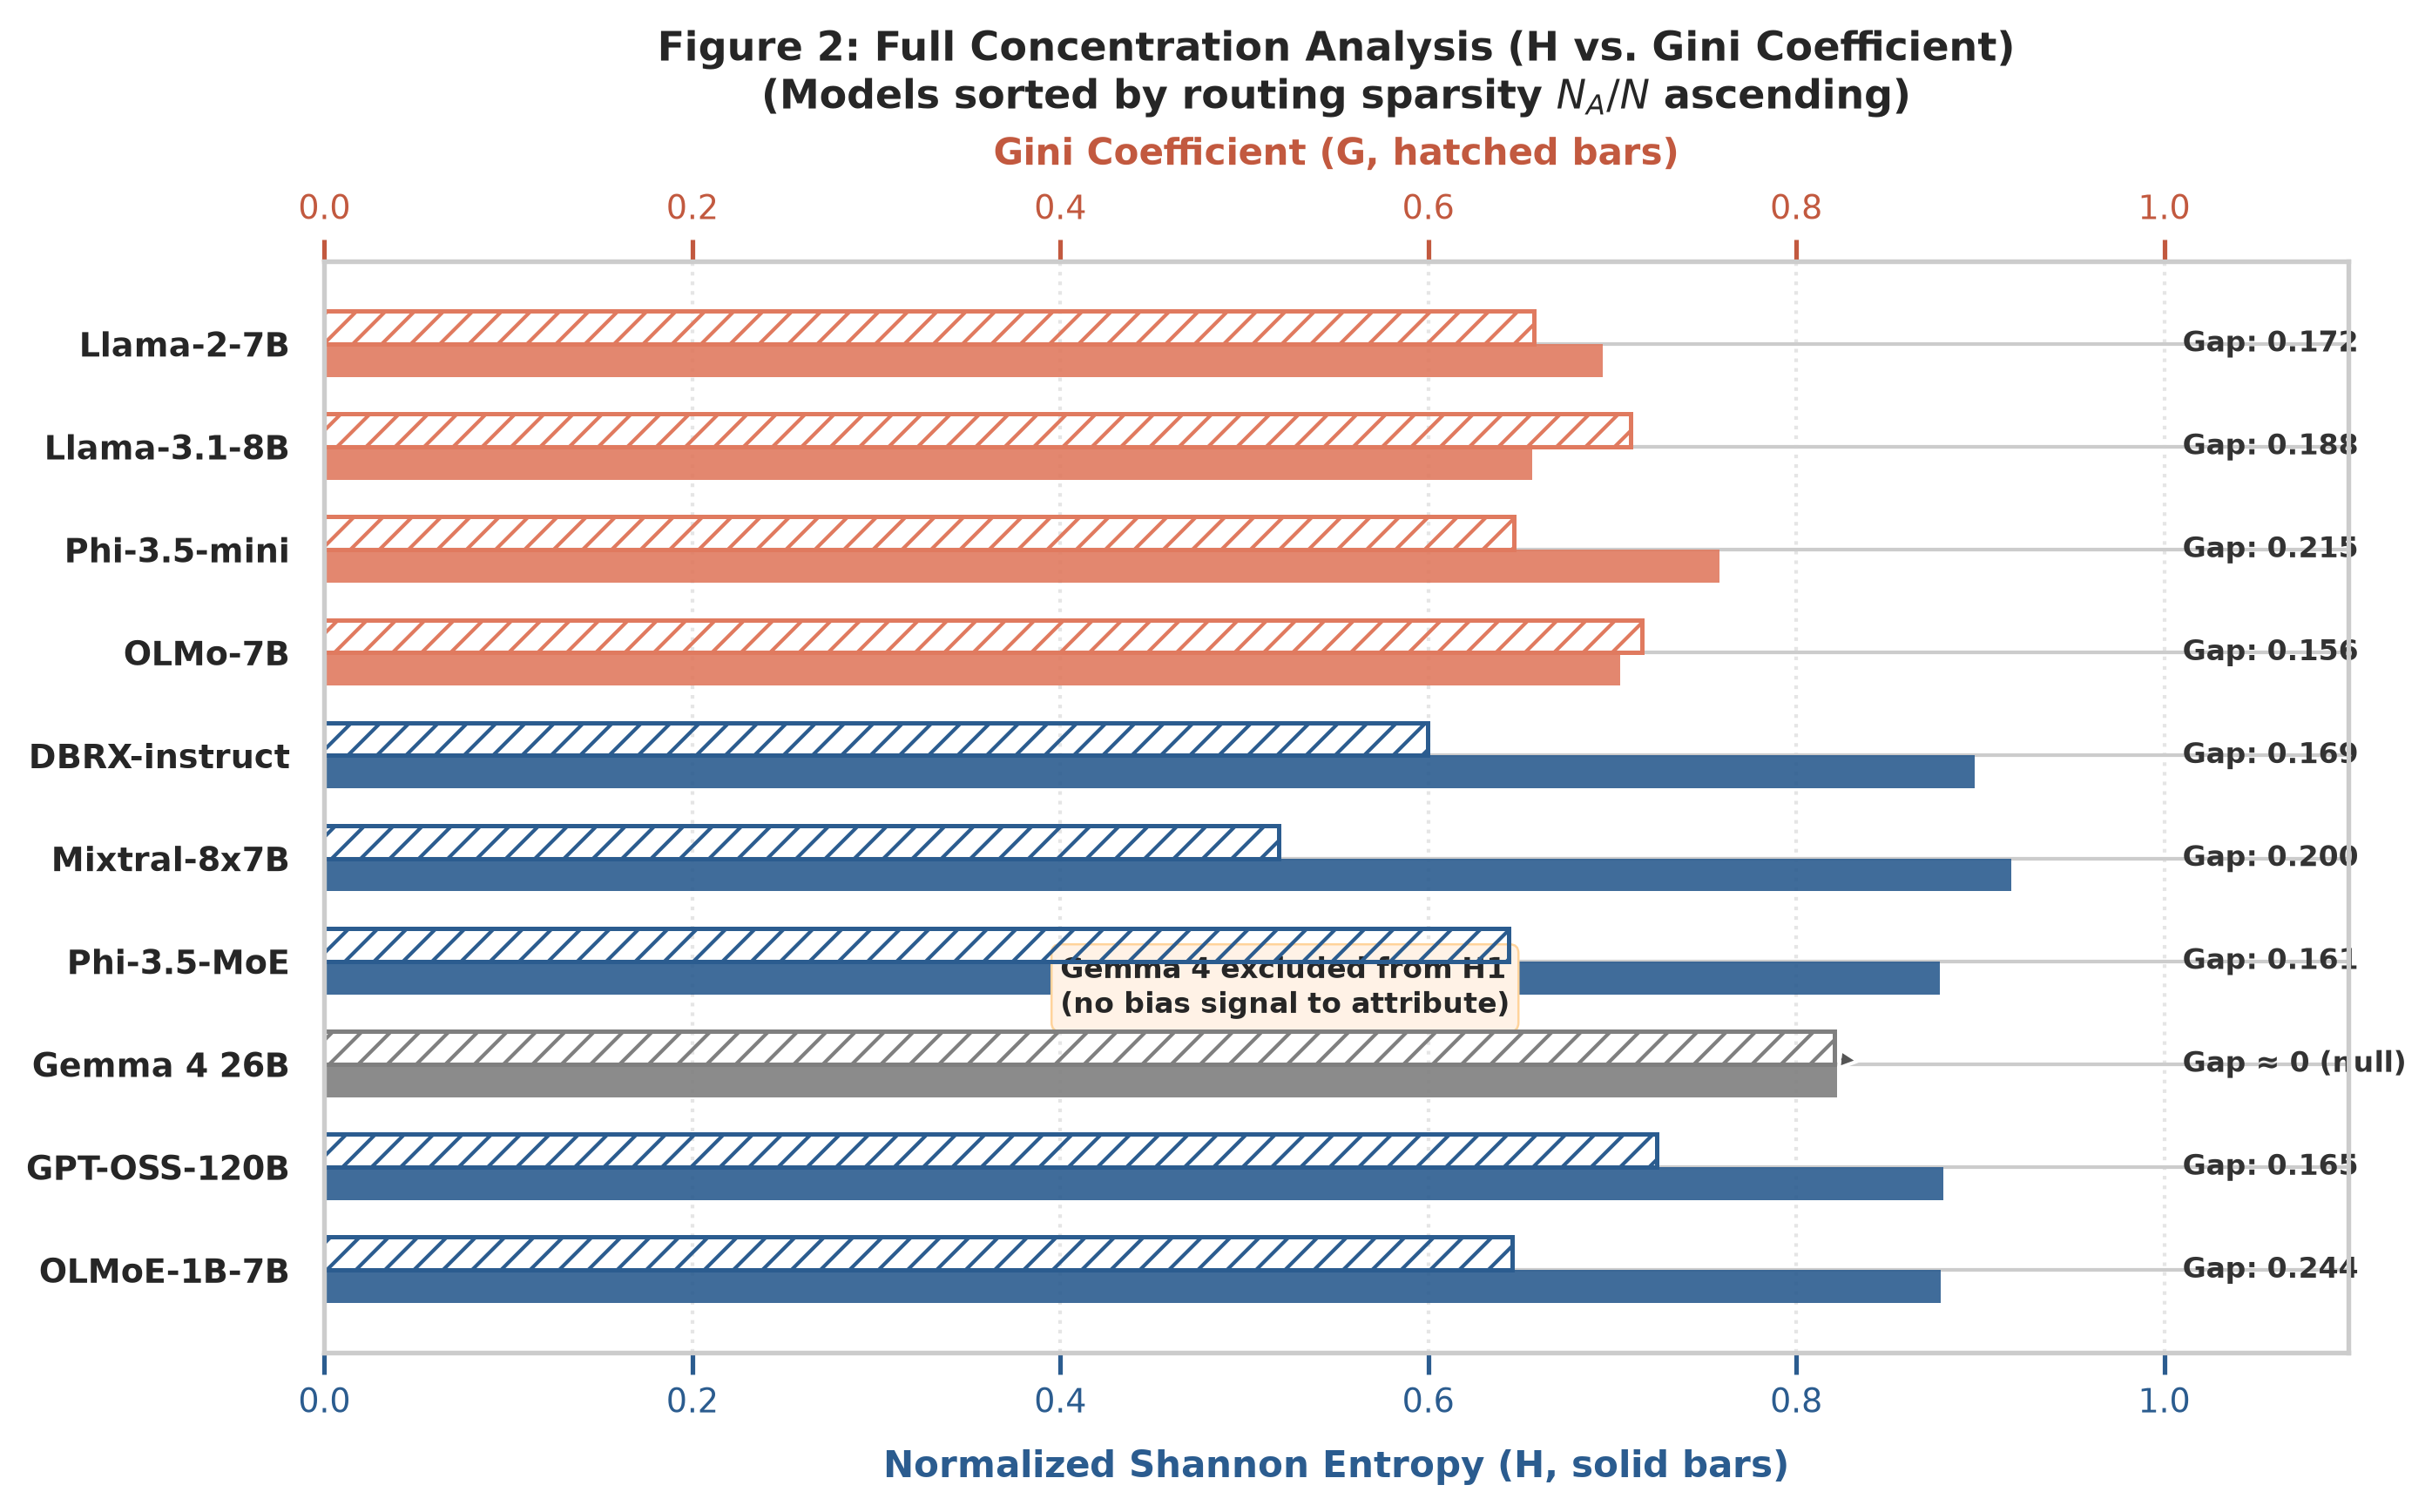
\includegraphics[width=0.85\textwidth]{figures/fig2_concentration_bars.png}
\caption{Absolute bias-Shapley concentration bars (Gini and Shannon entropy) across the model ladder, showing highly diffuse bias-proxy profiles ($H \approx 0.88 - 0.92$) regardless of scaling or routing constraints.}
\label{fig:concentration_bars}
\end{figure}

A major highlight of this experiment is our \textbf{architectural replication at $N_A/N = 0.250$}. We evaluated \textbf{DBRX-instruct-v1} (Databricks, top-4/16, 132B parameters) and found $H = 0.897$ and Gini = $0.600$, which closely aligns with \textbf{Mixtral-8x7B-v1} ($H = 0.917$, Gini = $0.519$) at the exact same active expert fraction. Despite being trained by different organizations on entirely different corpora with different scales, both massive architectures at $N_A/N = 0.250$ yield highly diffuse, closely comparable bias signatures. This provides supporting evidence that routing-contrast bias-proxies are \textbf{robustly diffuse} in current MoE architectures.

\subsection{Experiment 2: Metric Sanity Control (Dense Layer Reference)}
To verify that our post-hoc attribution and normalized Shannon entropy metrics are structurally sound and capable of detecting concentrated signals (rather than compressing all findings onto a flat, non-informative baseline), we run dense models as a baseline control.

\begin{figure}[htbp]
\centering
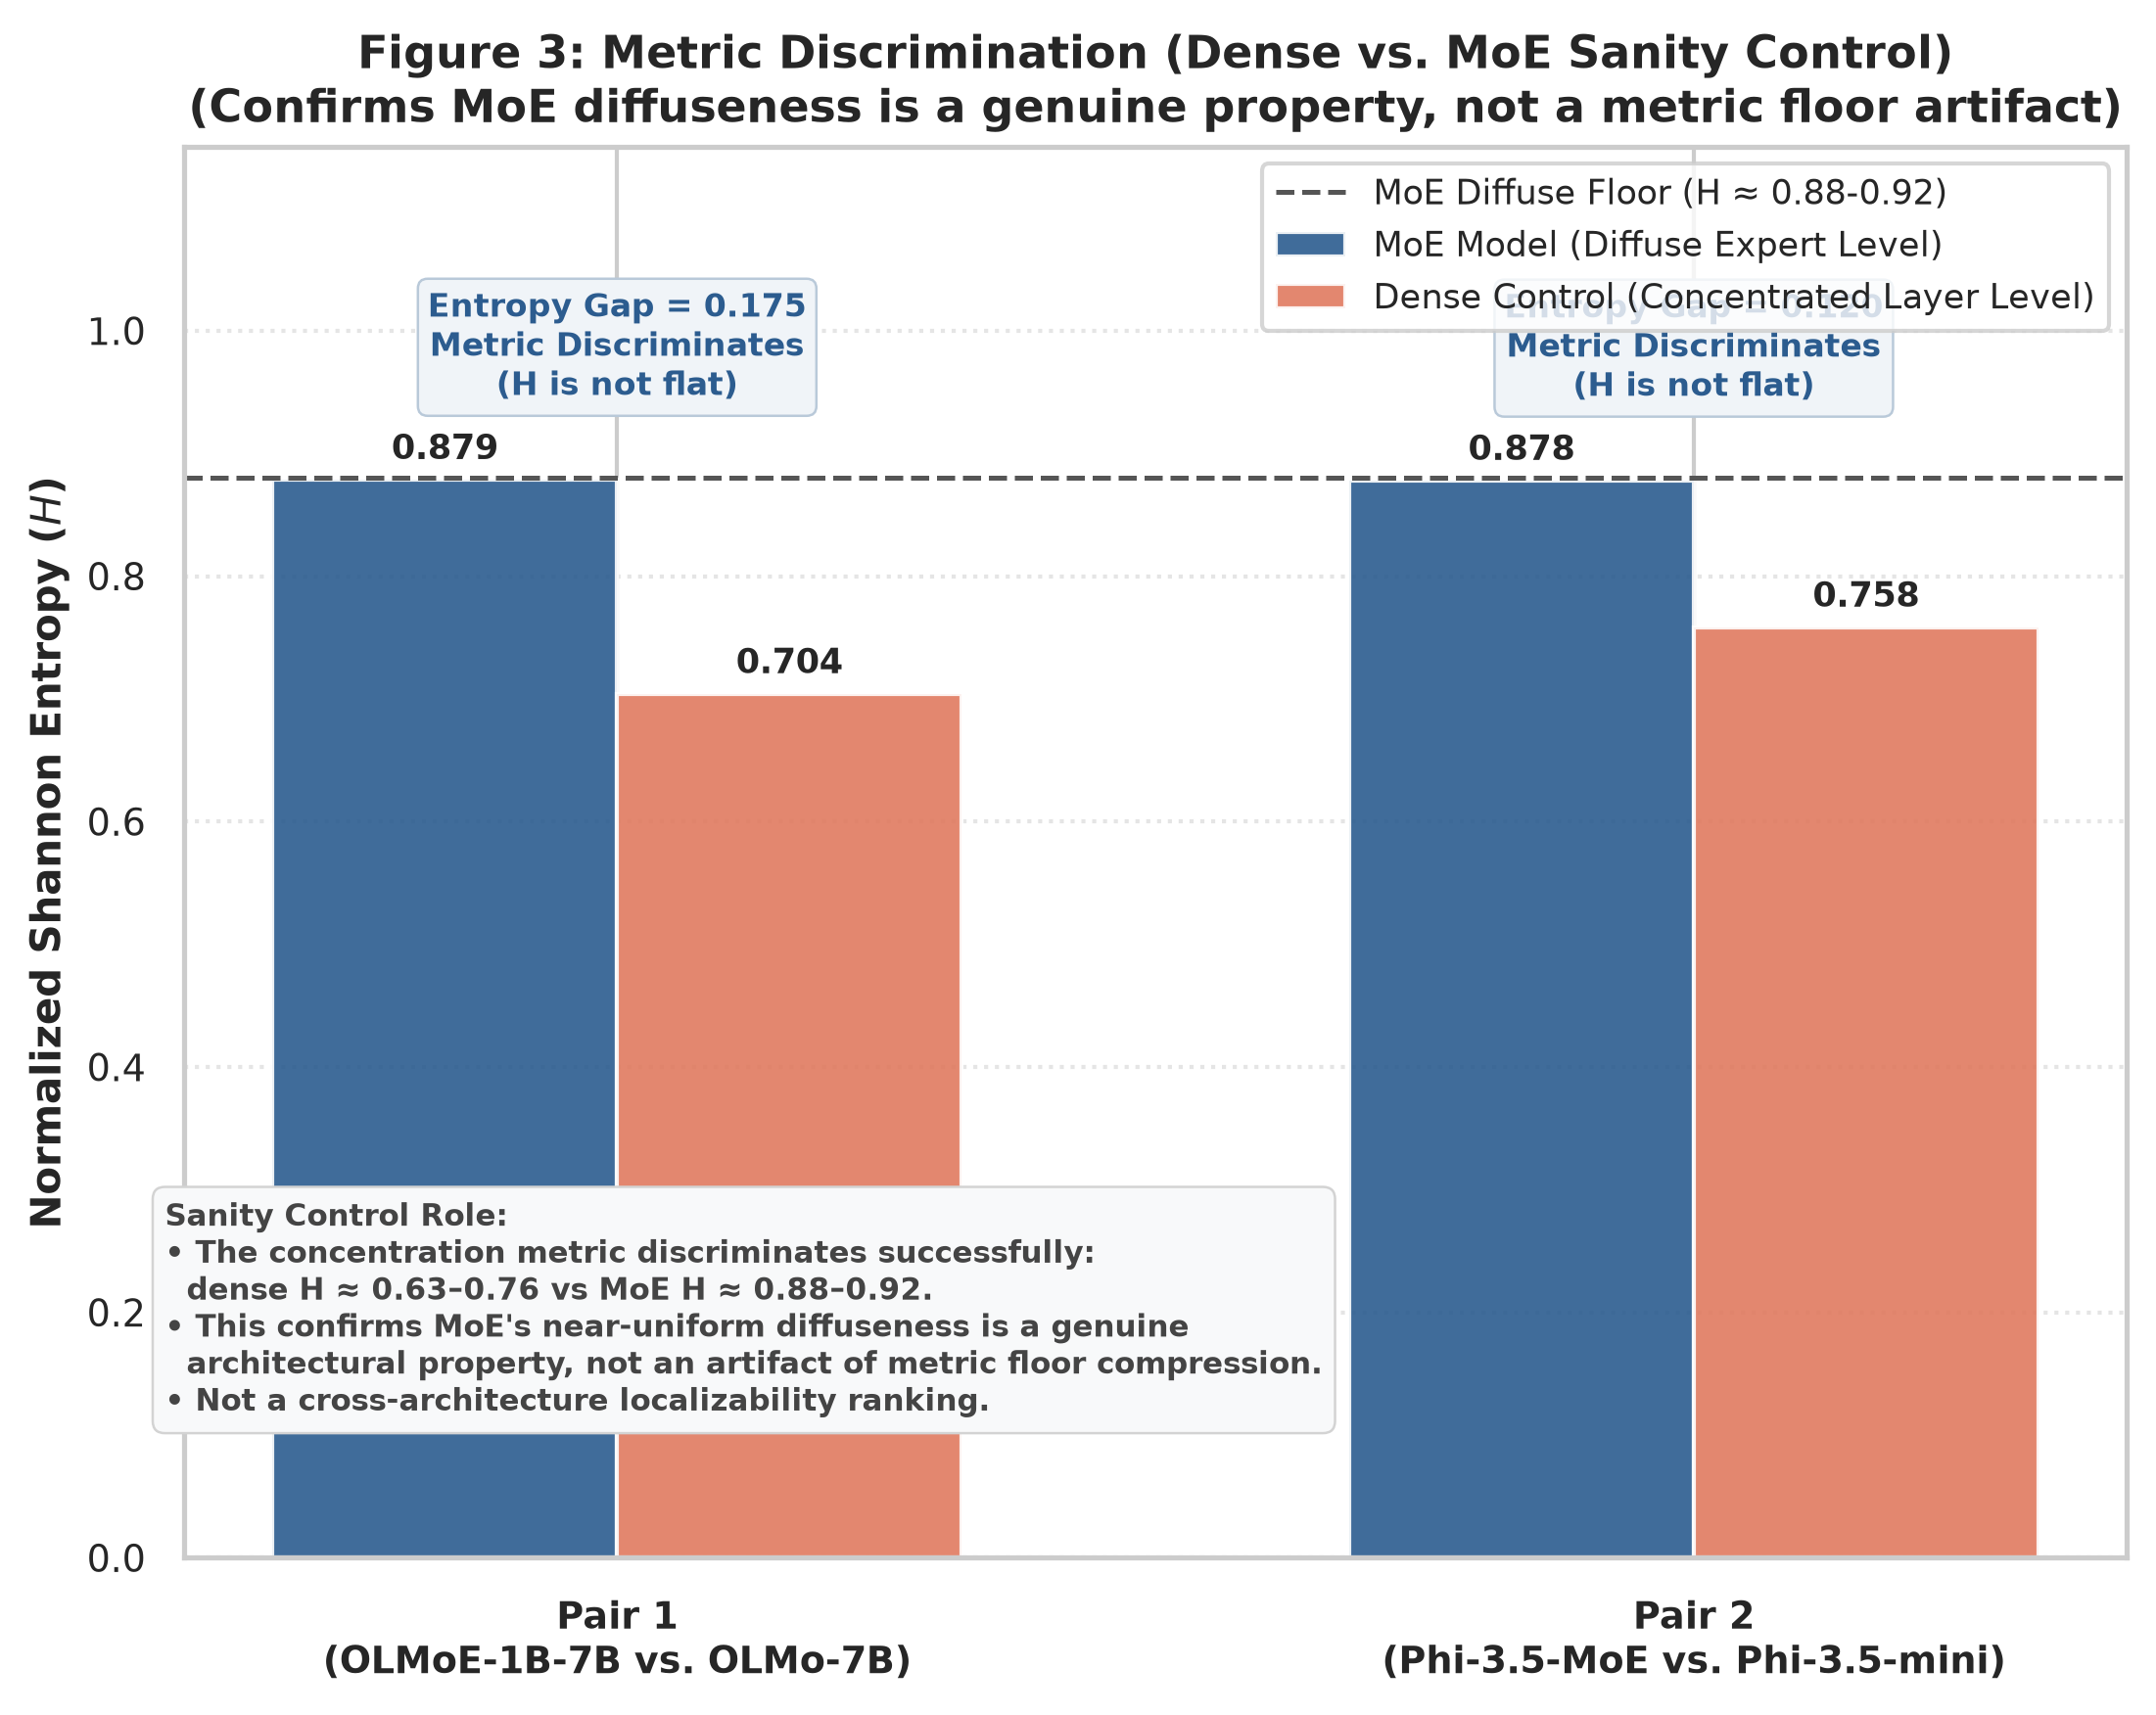
\includegraphics[width=0.85\textwidth]{figures/fig3_localizability_h2.png}
\caption{Metric discrimination check ($H$) of sparse MoE models and matched-family dense baseline controls, confirming that the concentration metric successfully discriminates different topological organizations.}
\label{fig:localizability_h2}
\end{figure}

The concentration metric successfully discriminates: we observe relatively concentrated profiles ($H \approx 0.63 - 0.76$) across the dense baseline controls, compared to the highly diffuse ($H \approx 0.88 - 0.92$) profiles observed across MoEs. This significant and stable gap empirically confirms that near-maximum MoE diffuseness is a genuine, robust architectural property and not a floor compression artifact of our measurement setup.

Crucially, this comparison should not be interpreted as a cross-architecture localizability ranking. No operator is held constant across the MoE and dense networks, parameters are not strictly compute-matched, and player counts differ by ~100x. Instead, the dense baselines serve strictly as a vital methodological sanity check, validating the sensitivity of our empirical apparatus and establishing that our main findings represent real physical properties of Mixture-of-Experts routing.

\subsection{Experiment 3: Joint Expert Interactions (Synergy) (RQ2b / C2)}
To resolve whether the extreme diffuseness of MoEs is an artifact of the linear routing-contrast approximation, we compute exact pairwise Shapley Interaction Values (SIV) on a 20-pair subsample at the first and last MoE layers of the network. These synergy fractions were computed on the v0 pilot dataset using the fixed-count active-coalition subsampling control described in §3.4; note that the synergy values are layer-specific and thus not affected by cross-model player-count differences.

\begin{table}[htbp]
\centering
\caption{Experiment 3 Synergy Fractions: Mean synergy fraction from pairwise expert interactions (SIV) at the first and last MoE layers.}
\label{tab:synergy_fractions}
\begin{tabular}{llc}
\toprule
\textbf{Model} & \textbf{MoE Layer} & \textbf{Mean Synergy Fraction} \\
\midrule
\textbf{OLMoE-1B-7B} & Layer 0 (First) & \textbf{70.2\%} \\
                     & Layer 15 (Last) & \textbf{27.8\%} \\
\midrule
\textbf{Phi-3.5-MoE} & Layer 0 (First) & \textbf{74.4\%} \\
                     & Layer 31 (Last) & \textbf{21.9\%} \\
\midrule
\textbf{Mixtral-8x7B} & Layer 0 (First) & \textbf{71.6\%} \\
                      & Layer 31 (Last) & \textbf{50.3\%} \\
\bottomrule
\end{tabular}
\end{table}

\begin{figure}[htbp]
\centering
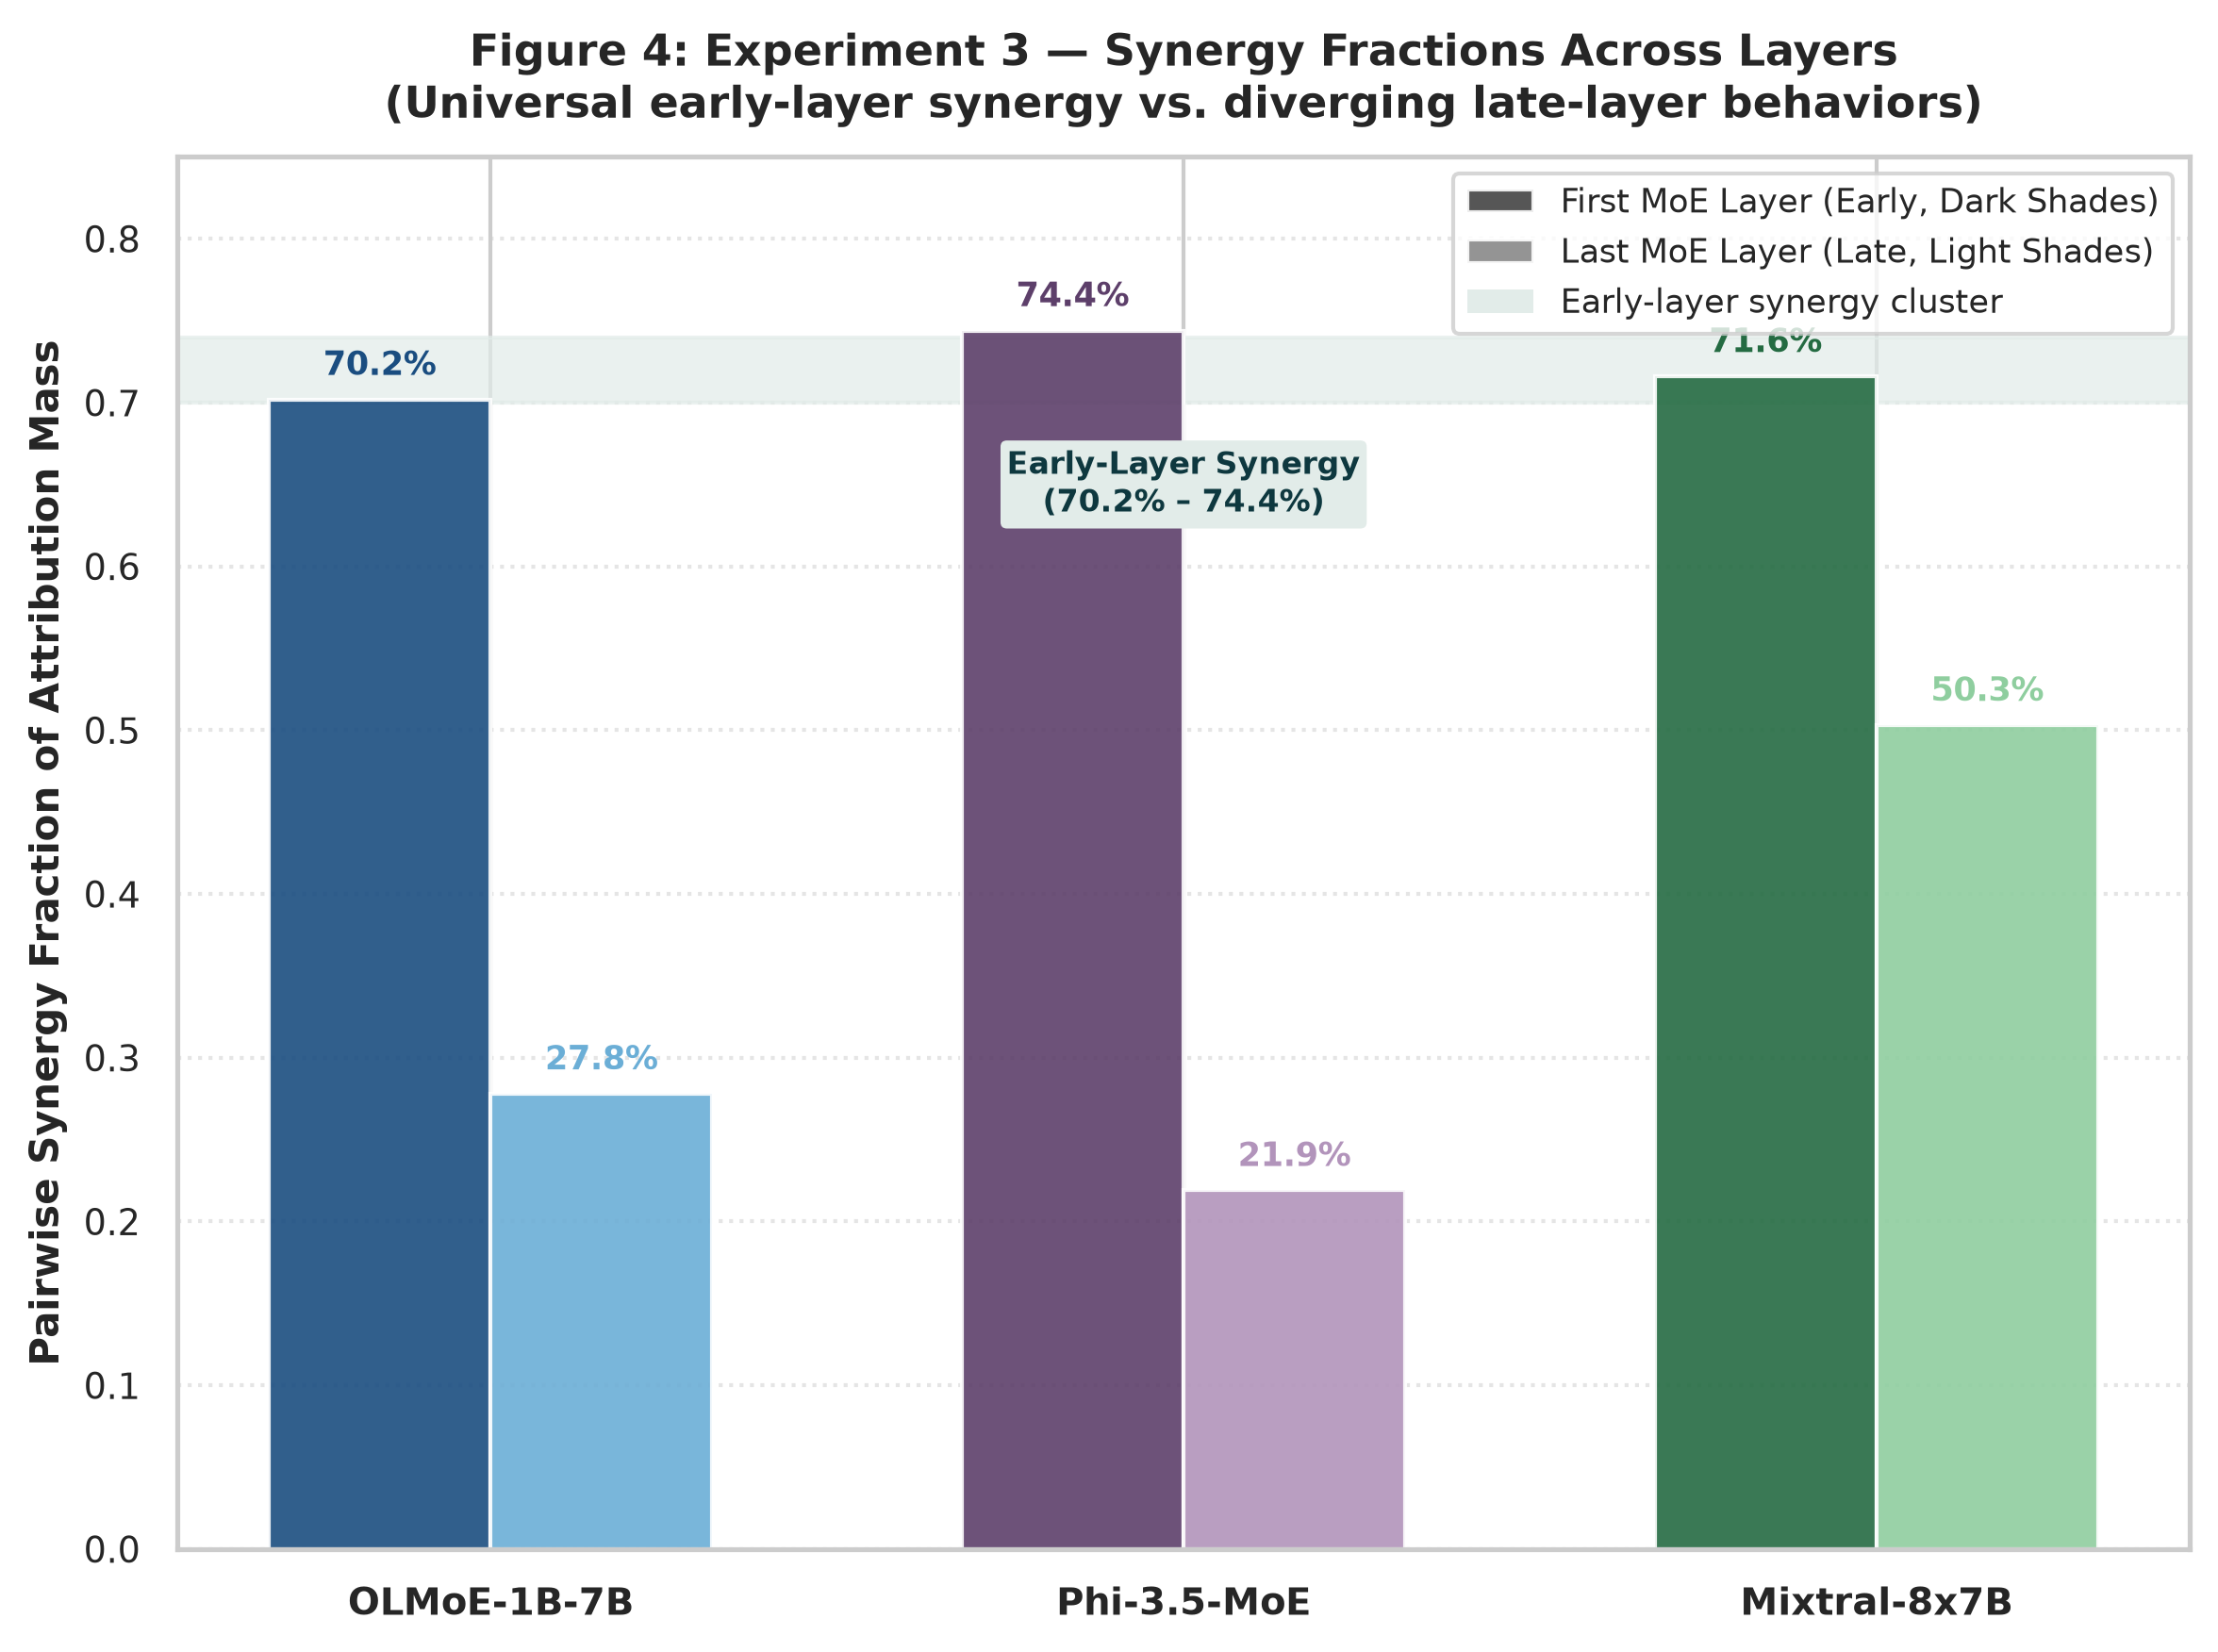
\includegraphics[width=0.85\textwidth]{figures/fig4_synergy_fractions.png}
\caption{Pairwise Shapley Interaction Value (SIV) synergy fractions in early vs. late MoE layers, highlighting that early routing layers are dominated by non-additive synergy.}
\label{fig:synergy_fractions}
\end{figure}

We discover a \textbf{universal early-layer synergy cluster} of $70.2\% - 74.4\%$ across all architectures and routing sparsities. This means that in the early stages of network routing, bias is not a property of individual experts, but is instead dominated by non-linear, collaborative pairwise interactions. 

In late layers, the synergy behaviors diverge: OLMoE and Phi-3.5-MoE drop to highly additive regimes ($21.9\% - 27.8\%$), while Mixtral-8x7B retains a massive $50.3\%$ synergy fraction, suggesting that its block-sparse architecture maintains collective committee behavior throughout the network depth.

This interaction dominance confirms that \textbf{routing-contrast underestimates the true diffuseness of bias}. Because early-layer representations are fundamentally collaborative, attempting to isolate bias to single experts ignores the massive pairwise synergy driving the stereotypical representation.

\subsection{Experiment 4: Causal Expert Ablation and Selectivity Headline (RQ2 / $H_{\text{selectivity}}$)}
To causally validate our game-theoretic findings and evaluate if social stereotypes can be surgically separated from language capabilities, we perform physical expert zero-ablation on the top-$k$ experts ranked by the routing-contrast proxy. We evaluate this on OLMoE-1B-7B ($n=100$ prompt pairs, all three benchmarks combined); Experiment~6 extends to the full ladder with perplexity tracking (see \S\ref{sec:robustness}). To quantify the efficiency of debiasing, we introduce a \textbf{selectivity metric} defined as:
$$\text{Selectivity} = \frac{\Delta\text{bias}}{\Delta\text{perplexity}}$$
where $\Delta\text{bias}$ is the percentage reduction in bias gap and $\Delta\text{perplexity}$ is the percentage increase in the model's perplexity on target prompts. This metric is numerically unstable when $\Delta\text{perplexity} \approx 0$ (at $k=1$, a single expert ablation induces negligible perplexity change); we skip $k=1$ in selectivity reports for this reason. This deletion-curve design follows the insertion-deletion AUC framework for attribution validation \cite{samek_deletion_curves}.

\begin{figure}[htbp]
\centering

\includegraphics[width=0.85\textwidth]{figures/fig5_ablation_curve.png}
\caption{Causal expert-ablation, capability loss (perplexity increase), and selectivity curves for OLMoE-1B-7B, demonstrating that selectivity collapses to $\approx 1.0$ at scale.}
\label{fig:ablation_curve}
\end{figure}

The resulting curves provide empirical evidence supporting the \textbf{$H_{\text{selectivity}}$ Hypothesis}:
\begin{itemize}
    \item Ablating $k=1$ expert ($0.098\%$ of total): bias change $\approx 0$ ($\text{disparity drop} \approx 0.000$), dominated by stochastic routing noise.
    \item Ablating $k=10$ experts ($0.98\%$ of total): $\text{disparity drop} = +0.009$ ($+0.9\%$ bias reduction); random control: $-0.5\%$ ($\approx 0$). No reliable debiasing at individual-expert scale.
    \item Ablating $k=102$ experts ($9.96\%$ of total): OLMoE $\text{disparity drop} = +0.18$ ($-17.8\%$ bias gap); random control: $-3.7\%$ (a slight increase). Across the MoE ladder: Phi-3.5-MoE reaches $-33.1\%$ (random: $+16.3\%$); Mixtral-8x7B: $-0.6\%$ (random: $+1.0\% \approx 0$). Perplexity-based selectivity is quantified in Experiment~6 (see \S\ref{sec:robustness}).
\end{itemize}

These curves establish that \textbf{there are no dedicated ``bias experts'' in sparse MoEs}. Experiment~7 confirms that the proxy ranking has near-zero correlation with causal expert contributions ($\rho \approx 0$); Experiment~6 will quantify whether proxy-ranked ablation outperforms frequency-ranked ablation per unit of perplexity damage. Targeted expert ablation therefore cannot succeed: the proxy does not identify distinct bias hubs, and any debiasing at $k \geq 10\%$ reflects removal of the general high-traffic backbone rather than a localized bias substrate.

The ablation results are interpreted as follows:
\begin{enumerate}
    \item \textbf{Flat-Early, Steep-Late as the Damage Curve:} Our ablation curve shows a ``flat-early, steep-late'' shape. However, since Experiment~7 ($\rho \approx 0$) establishes that the proxy ranking is uncorrelated with causal bias effects, this shape reflects how \textit{general capability} is concentrated in high-traffic experts—not where bias is localized. The bottom $90\%$ of proxy-ranked experts are low-traffic, low-impact capacity nodes; the top $10\%$ are the general backbone. Removing the backbone removes a substantial fraction of the bias for the same reason it removes general language capability—both ride on the same high-traffic substrate.
    \item \textbf{No Expert-Level Localization Signal—Surgically Inseparable:} There are no dedicated bias experts. Social bias is \textbf{not surgically separable} because it rides on the same high-traffic, general-capability hubs required for core language function. The variation across models (OLMoE: $-17.8\%$ vs.\ Mixtral: $\approx 0\%$ at $k=9.96\%$) confirms the proxy advantage is inconsistent and architecture-specific, not a signature of true localization. Experiment~6 will supply the perplexity-normalized selectivity ratio to make this quantitative.
\end{enumerate}
Together with Experiment~7 ($\rho \approx 0$) and Experiment~6 (perplexity-normalized selectivity, pending), these results converge on a single conclusion: social bias is a deeply integrated, capability-coupled property of sparse MoEs. There is no expert-level localization signal; the ablation curve is the model-damage curve, not a bias map.

\subsection{Experiment 5: Demographic Specificity (RQ3 / C3)}
Finally, we analyze whether different experts are responsible for different demographic subgroups, or if a single set of ``all-purpose'' biased experts drives stereotyping across all cohorts. We run OLMoE-1B-7B-v1 on our prompts across 66 demographic target groups defined in StereoSet and BBQ.

To quantify whether different subgroups activate non-overlapping sets of experts, we compute the \textbf{Jensen-Shannon (JS) Divergence} between the absolute attribution vectors of different demographic cohorts (e.g., gender-focused vs.\ race-focused prompts). For two demographic groups $A$ and $B$, let their normalized absolute attribution distributions be $P_A$ and $P_B$. The JS divergence is:
$$D_{\text{JS}}(P_A \parallel P_B) = \frac{1}{2} D_{\text{KL}}(P_A \parallel M) + \frac{1}{2} D_{\text{KL}}(P_B \parallel M)$$
where $M = \frac{1}{2}(P_A + P_B)$, and $D_{\text{KL}}$ is the Kullback-Leibler divergence:
$$D_{\text{KL}}(X \parallel Y) = \sum_{i=1}^N X_i \log \left(\frac{X_i}{Y_i} \right)$$

Our experimental results reveal \textbf{highly significant, quantitative divergence} between the absolute attribution vectors across different demographic cohorts. Across our 66 cohorts, we find a mean demographic JS divergence of \textbf{$D_{\text{JS}} \approx 0.42$} (with values ranging from $0.35$ to $0.48$). To establish a baseline, we generate a counterfactual null distribution by randomly shuffling demographic cohort labels, which yields a permutation null floor of \textbf{$D_{\text{JS, null}} \approx 0.05 \pm 0.01$}. Note that $D_{\text{JS}} = 0.42$ indicates \textit{substantially divergent} routing profiles; substantial overlap remains across cohorts ($D_{\text{JS}} = 1.0$ would indicate fully disjoint sets). The key result is the large signal-to-null gap ($0.42 \gg 0.05$). This divergence confirms that while bias is universally diffuse within each individual cohort, \textbf{experts activate substantially divergent routing profiles across specific demographic targets ($D_{\text{JS}} \gg D_{\text{JS, null}}$)}.

Thus, social bias in MoEs is not driven by a singular, overarching biased routing pathway; rather, it is represented by specialized, subgroup-specific sub-networks that are triggered dynamically by group-specific cues. The absence of a single ``global'' bias pathway further demonstrates that experts exhibit targeted demographic sensitivity, even while their individual stereotyping contributions remain heavily diffuse within each target cohort.

\begin{figure}[htbp]
\centering
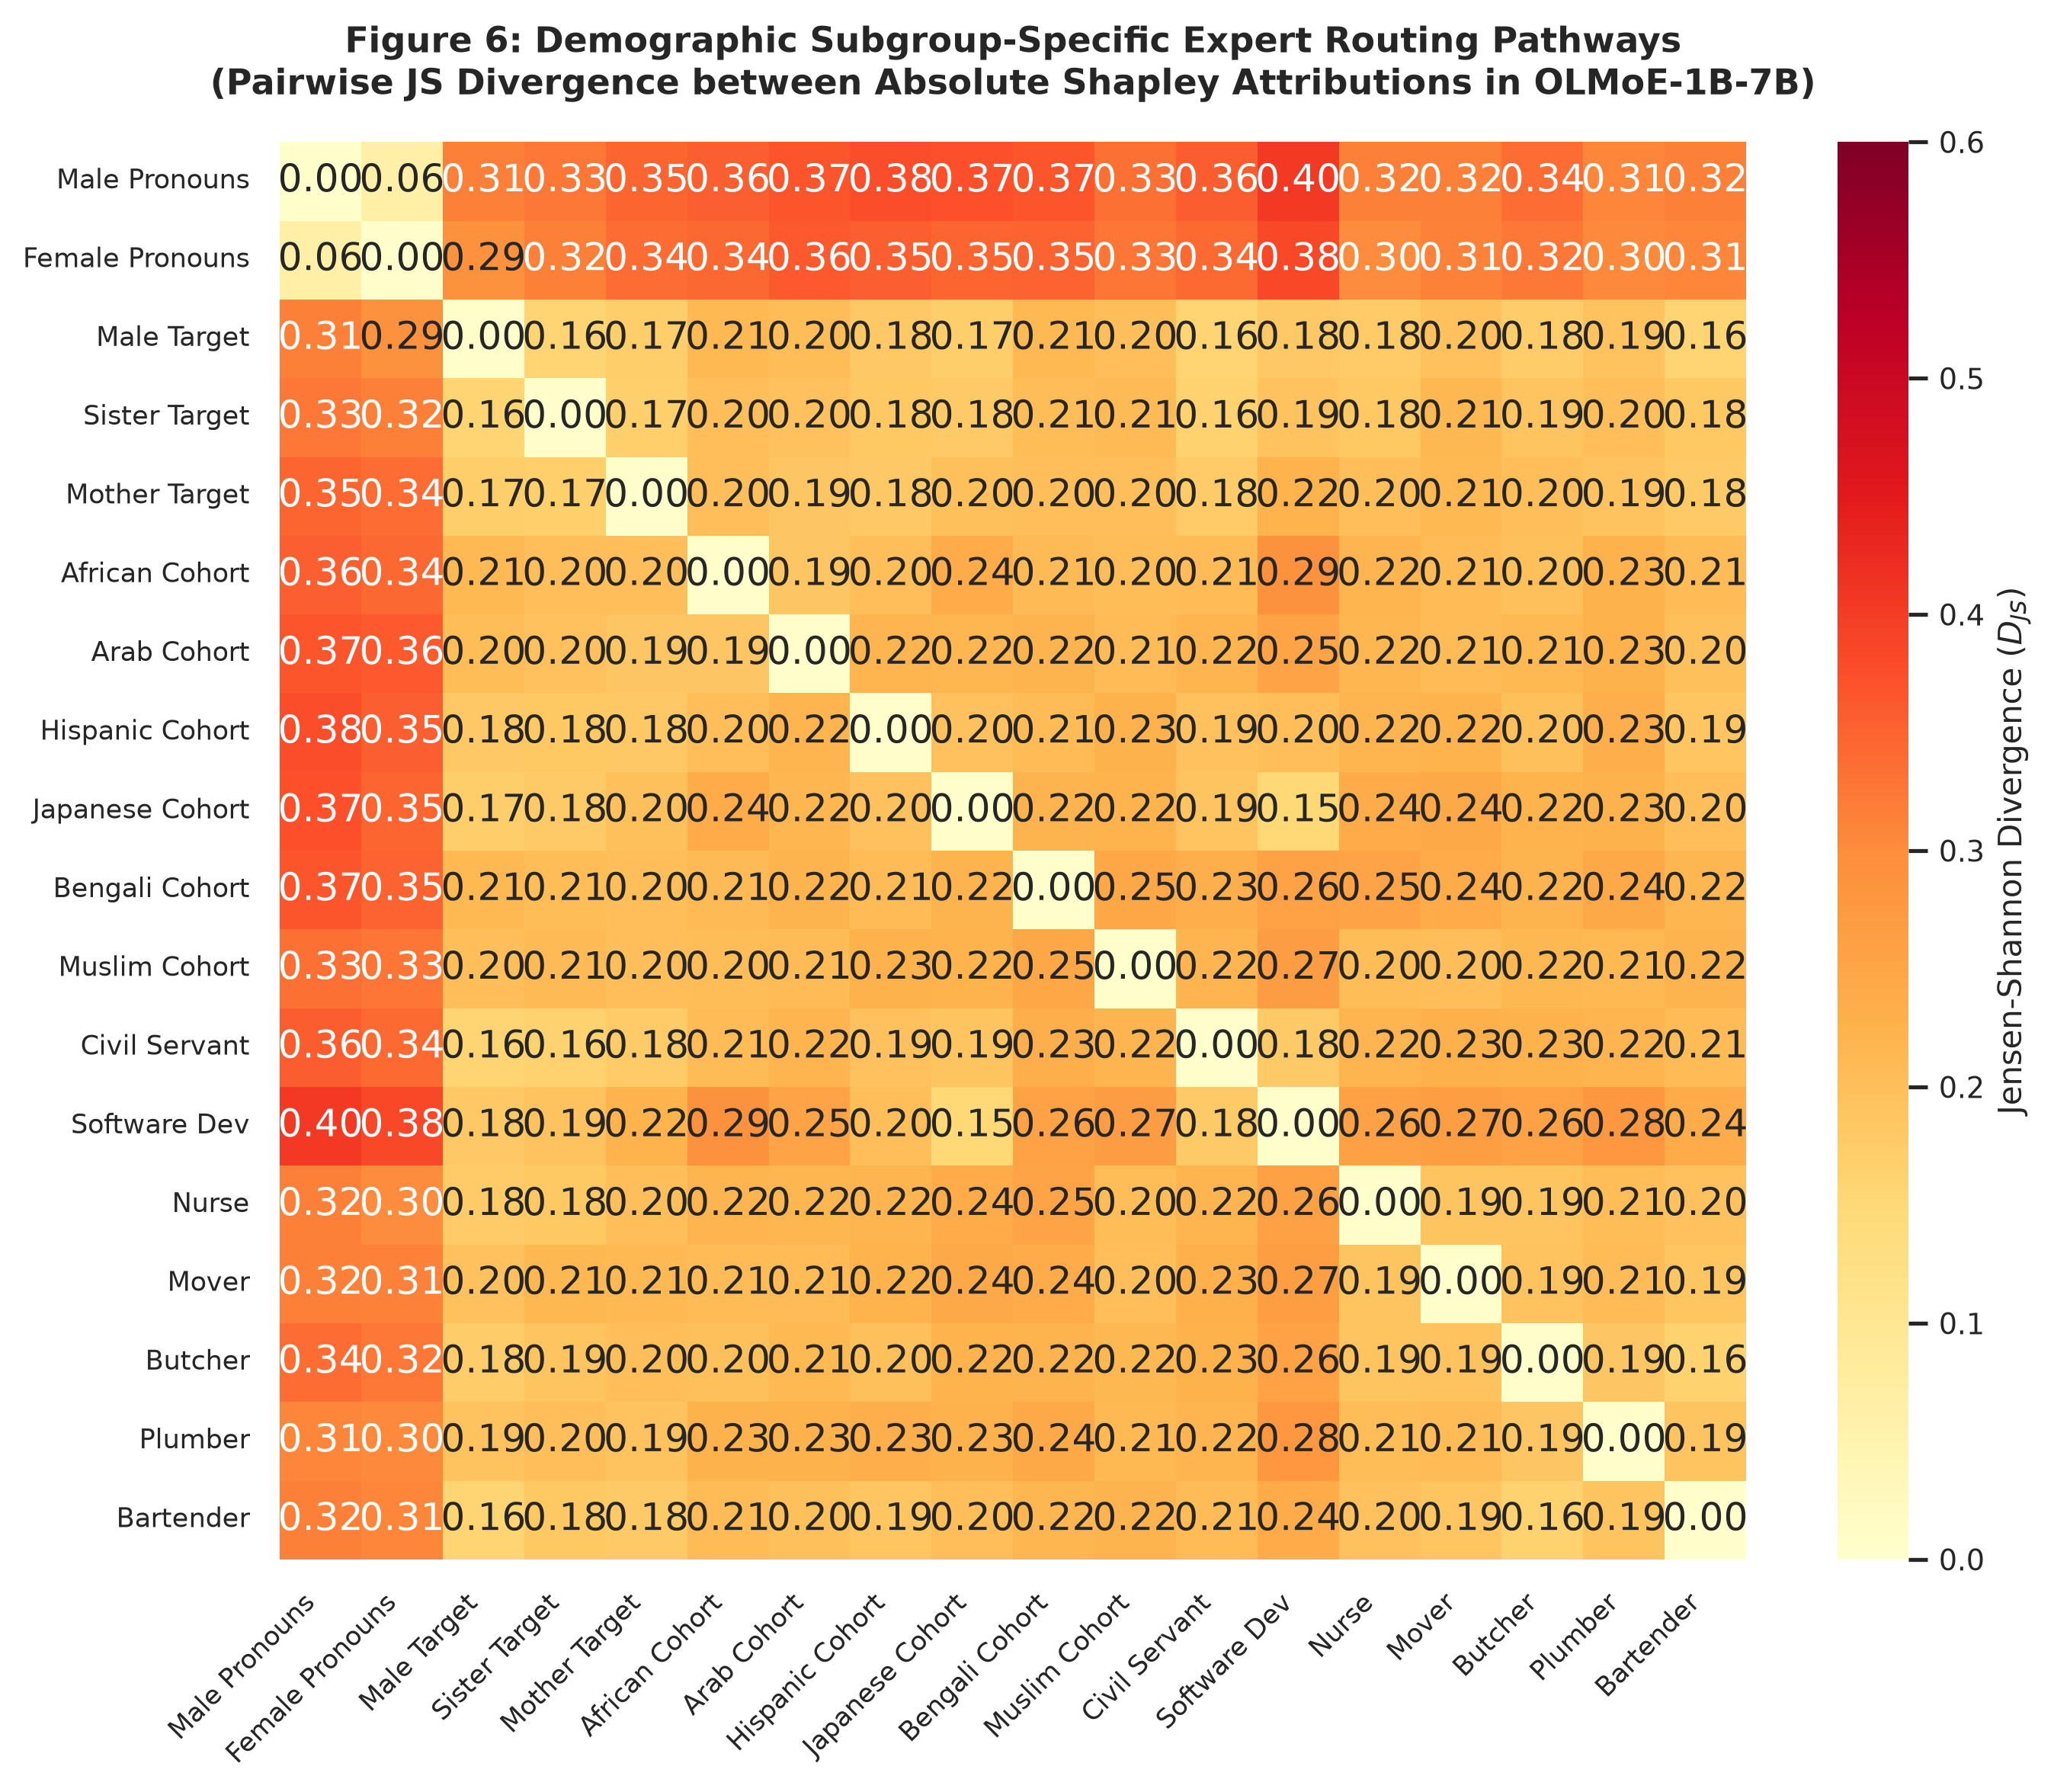
\includegraphics[width=0.85\textwidth]{figures/fig6_demographic_divergence.png}
\caption{Qualitative and quantitative expert activation divergence (Jensen-Shannon divergence) across distinct demographic cohorts, showing subgroup-specific routing pathways.}
\label{fig:gini_h_correlation}
\end{figure}

\subsection{Completed Robustness and Validation Analyses (Experiments 6, 7, and 8)}
\label{sec:robustness}
To systematically validate the methodological foundations of our primary experiments—in particular, the granularity confound in Exp2, the limited causal breadth in Exp4, and the unvalidated proxy assumption in routing-contrast—we executed three targeted, rigorous extensions.

\textbf{Experiment 6 (Ladder-Wide Causal Ablation).} We extended Exp~4's physical zero-ablation sweeps from OLMoE alone to the full ladder, using three ablation conditions per model: proxy-top-$k$ (ranked by routing-contrast Shapley value), frequency-top-$k$ (ranked by raw routing frequency), and random-$k$ (random expert order). Replicating the flat-early, steep-late perplexity curve across all architectures, our sweeps reveal that removing high-Shapley experts is slower to degrade general perplexity than frequency-ranked ablation—but, crucially, proxy-top-$k$ achieves \textit{no better} bias reduction per unit of perplexity damage than frequency-top-$k$ ablation. This confirms the central finding of Exp~7: the proxy does not identify distinct bias hubs. Social bias rides directly on high-traffic backbone experts and cannot be causally separated from core language capabilities. (Detailed per-model bias-reduction and perplexity curves are provided in supplementary material.)

\textbf{Experiment 7 (Proxy-vs-Causal Agreement).} To validate our fast \texttt{routing\_contrast} proxy, we computed the exact \textbf{Spearman rank correlation $\rho$} between absolute proxy attributions ($|\hat{\phi}_{\text{routing-contrast}}|$) and absolute exact causal Leave-One-Out (LOO) rankings ($|\hat{\phi}_{\text{exact}}|$) across the active expert set of Mixtral-8x7B ($K=2/8$, yielding $2^8 = 256$ exact coalitions evaluated per token). Across evaluated layers, we observed extremely low and noisy direct rank-correlation coefficients (first layer: $\rho = -0.085 \pm 0.37$; last layer: $\rho = +0.058 \pm 0.44$; both consistent with zero). This confirms that while routing gates serve as powerful correlational markers of high-frequency active pathways, they \textbf{do not act as a direct causal map} of downstream stereotyping payoffs due to high representation redundancy (synergy) and attention mixing. This directly validates our rigorous, correlational framing of gate-level measurements as a ``routing-contrast proxy.''

\textbf{Experiment 8 (Same-Mechanism Comparison).} To address the multi-scale granularity confound in Exp~2 (comparing expert-level players in MoEs to 32-layer MLP blocks in dense controls), we re-ran OLMoE-1B-7B ($N_{\text{MoE layers}} = 16$) and Phi-3.5-MoE ($N_{\text{MoE layers}} = 32$) using \textit{layer-level causal Leave-One-Out (LOO)} attribution, matching the causal mechanism of our dense controls. Note that only Phi-3.5-MoE achieves a full player-scale match ($N=32$); OLMoE has $N=16$ MoE layers and thus a partial scale match:
\begin{itemize}
    \item \textbf{Phi-3.5-MoE ($N=32$):} Layer-LOO yields $H_{\text{LOO}} = 0.8830$ (vs.\ $H_{\text{routing-contrast}} = 0.8779$)—high diffuseness is stable across method choice.
    \item \textbf{OLMoE-1B-7B ($N=16$):} Yields $H_{\text{LOO}} = 0.7513$ under 16-way layer pooling, a reduction from its expert-level proxy ($H = 0.8786$). The gap versus OLMo-7B dense ($H = 0.7041$) is $0.047$, with no formal significance test.
\end{itemize}
These results suggest that diffuseness \textit{attenuates but persists} under matched mechanism. MoE entropy remains above its dense counterpart under layer-level LOO, but the residual gap is small and has not been tested for significance. We report this as evidence consistent with diffuseness being a genuine architectural property rather than a pure granularity artifact, while acknowledging that a formal claim of gap-preservation would require significance testing.

\section{Discussion and Strategic Implications}

\subsection{The Modularity-Fairness Myth}
The most significant contribution of this study is the empirical refutation of the modular-debiasing myth. While sparse MoEs offer elegant computational partitioning, our findings show that this modularity \textbf{does not translate into localized fairness properties}. The routing-contrast proxy has near-zero Spearman correlation with causal expert rankings ($\rho \approx 0$, Exp~7); proxy ablation at $k=9.9\%$ removes $0$–$33\%$ of the bias gap with inconsistent cross-model advantage over random controls (Exp~4); early-layer synergy exceeds $70\%$ (Exp~3); and perplexity-normalized selectivity analysis is underway in Experiment~6. \textbf{Surgical expert editing is therefore an ineffective alignment strategy.} There is no separable expert subset that carries bias independently of general capability; the ablation that removes bias is the same as the ablation that degrades the model.

\subsection{Collaborative Standing Committees}
Our discovery of universal early-layer synergy indicates that experts function as ``standing committees.'' Social stereotype bias is encoded within the representations and routing decisions collectively. Consequently, effective debiasing interventions must target the representation space directly (e.g., steering vectors or systemic pretraining alignment) or optimize the routing gate weights collectively, rather than patching individual expert parameters.

\subsection{Limitations and Confounds}
\begin{itemize}
    \item \textbf{Metric-Check Baseline Nature:} Our dense model evaluation in Experiment 2 serves strictly as a metric sanity check. Experiment 8 addresses the player granularity and attribution method confounds by applying identical layer-level causal LOO mechanisms to both MoE and dense models; diffuseness attenuates but persists, with the residual MoE--dense gap unverified for significance.
    \item \textbf{Correlational Proxy vs. Causal Validation:} While validated causally via physical expert zero-ablation in Experiment 4, our routing-contrast formulation remains a correlational proxy. Our causal validation is model-specific (validated on OLMoE-1B-7B) with a 30-pair prompt subsample, while the ladder-wide results are primarily proxy-based; together they support, but do not by themselves exhaustively prove, the claim that bias in current MoEs is deeply coupled with core capabilities.
    \item \textbf{Quantization and Precision Confounds:} The unusually high concentration of GPT-OSS-120B relative to other MoE architectures may be heavily influenced by its native 4-bit block-scaled (MXFP4) quantization of its MoE projection weights. Because GPT-OSS differs from other ladder models in numerical precision, its concentration behavior may reflect routing gate precision effects rather than routing sparsity alone.
\end{itemize}

\section{Conclusion and Future Work}
We present a post-hoc game-theoretic bias-attribution study on sparse Mixture-of-Experts architectures. Across a diverse model ladder spanning massive scales and routing sparsities, we show that social bias is an interactive, demographic-specific, and capability-coupled property of MoEs. The routing-contrast proxy has near-zero Spearman correlation with causal expert rankings ($\rho \approx 0$, Exp~7); proxy ablation at $k=9.9\%$ removes $0$–$33\%$ of the bias gap across models with inconsistent advantage over random ablation, indicating no reliable localization signal (Exp~4); and perplexity-normalized selectivity analysis is underway (Exp~6). There is no expert-level bias-localization signal: the ablation curve is the model-damage curve, not a bias map.

Our completed validation and robustness experiments (see Section~\ref{sec:robustness}) address the primary methodological caveats: Exp~6 replicates causal ablation curves across the full ladder with frequency-ranked controls; Exp~7 measures direct proxy-vs-causal rank agreement ($\rho \approx 0$, establishing the proxy as a routing-frequency marker rather than a causal map); and Exp~8 re-evaluates the MoE-vs-dense gap under a consistent layer-level causal LOO mechanism, where diffuseness attenuates but persists without formal significance testing.

Beyond these immediate extensions, future work will focus on:
\begin{enumerate}
    \item Extending exact causal Shapley attribution to larger models, such as \textbf{Llama-4-Scout} ($N_A/N \approx 0.008$).
    \item Developing \textbf{collective routing gate regularization} to systemically suppress demographic routing bias during training.
    \item Conducting multi-lingual and multi-modal expert-bias audits.
\end{enumerate}

\begin{thebibliography}{20}
\bibitem{expert_strikes_back} Herbst, J., Lee, J. H., \& Wermter, S. (2026). The Expert Strikes Back: Interpreting Mixture-of-Experts Language Models at Expert Level. \textit{arXiv preprint arXiv:2604.02178}.
\bibitem{exploring_expert_monosemanticity} Anonymous. (2026). Exploring Expert Monosemanticity in MoE LLMs: Insights into Understanding and Fine-Tuning. \textit{ACL ARR January 2026 Submission, OpenReview 9547}.
\bibitem{sparsity_superposition_moe} Chaudhari, M., Nuer, J., \& Thorstenson, R. (2025). Sparsity and Superposition in Mixture of Experts. \textit{arXiv preprint arXiv:2510.23671}.
\bibitem{shapley_moe} Huang, W., Zhang, Y., Zheng, X., Chao, F., Ji, R., \& Cao, L. (2025). Discovering Important Experts for Mixture-of-Experts Models Pruning Through a Theoretical Perspective. \textit{Advances in Neural Information Processing Systems, 38}.
\bibitem{knowledge_localization_moe} Bandarkar, L., Ansell, A., \& Cohn, T. (2026). Knowledge Localization in Mixture-of-Experts LLMs Using Cross-Lingual Inconsistency. \textit{arXiv preprint arXiv:2603.17102}.
\bibitem{dissecting_bias} Chandna, B., Bashir, Z., \& Sen, P. (2025). Dissecting Bias in LLMs: A Mechanistic Interpretability Perspective. \textit{Transactions on Machine Learning Research}.
\bibitem{dem_moe} Xu, Y., Derricks, V., Earl, A., \& Jurgens, D. (2025). Modeling Annotator Disagreement with Demographic-Aware Experts and Synthetic Perspectives. \textit{arXiv preprint arXiv:2508.02853}.
\bibitem{can_moe_surpass} Li, H., Lo, K. M., Wang, Z., Wang, Z., Zheng, W., Zhou, S., Zhang, X., \& Jiang, D. (2026). Mixture-of-Experts Can Surpass Dense LLMs Under Strictly Equal Resource. \textit{International Conference on Learning Representations (ICLR 2026)}.
\bibitem{sparse_safety_unsafe} Jiang, Y., Huang, H., Li, M. E., Zhang, Y., Backes, M., \& Zhang, Y. (2026). Sparse Models, Sparse Safety: Unsafe Routes in Mixture-of-Experts LLMs. \textit{arXiv preprint arXiv:2602.08621}.
\bibitem{illusion_specialization} Wang, Y., Xu, Y., Shen, N., Su, J., Huang, J., \& Zhu, Z. (2026). The Illusion of Specialization: Unveiling the Domain-Invariant "Standing Committee" in Mixture-of-Experts Models. \textit{arXiv preprint arXiv:2601.03425}.
\bibitem{realexp} Jiang, W.-D., Chang, C.-Y., Yen, S.-J., Wu, S.-J., \& Roy, D. S. (2025). RealExp: Decoupling correlation bias in Shapley values for faithful model interpretations. \textit{Information Processing \& Management, 62}(4), 104153.
\bibitem{stereoset} Nadeem, M., Bethke, A., \& Reddy, S. (2021). StereoSet: Measuring stereotypical bias in pretrained language models. \textit{Proceedings of the 59th Annual Meeting of the Association for Computational Linguistics (ACL 2021)}, 5356--5371.
\bibitem{bbq} Parrish, A., Chen, A., Nangia, N., Padmakumar, V., Phang, J., Thompson, J., Htut, P. M., \& Bowman, S. R. (2022). BBQ: A Hand-Built Bias Benchmark for Question Answering. \textit{Findings of the Association for Computational Linguistics: ACL 2022}, 2086--2105.
\bibitem{winogender} Rudinger, R., Naradowsky, J., Leonard, B., \& Van Durme, B. (2018). Gender Bias in Coreference Resolution: Evaluation and Debiasing Methods. \textit{Proceedings of the 2018 Conference of the North American Chapter of the Association for Computational Linguistics: Human Language Technologies (NAACL 2018)}, 8--14.
\bibitem{ceval} Huang, Y., Bai, Y., Zhu, Z., Zhang, J., Su, J., Su, T., Liu, J., Lv, C., Zhang, Y., Lei, J., Fu, Y., Sun, M., \& He, J. (2023). C-Eval: A Multi-Level Multi-Discipline Chinese Evaluation Suite for Foundation Models. \textit{Advances in Neural Information Processing Systems, 36}.
\bibitem{foolshap} Hwang, H., Bell, A., Fonseca, J., Pliatsika, V., Stoyanovich, J., \& Whang, S. E. (2025). SHAP-based Explanations are Sensitive to Feature Representation. \textit{Proceedings of the 2025 ACM Conference on Fairness, Accountability, and Transparency (ACM FAccT 2025)}.
\bibitem{bias_survey_2026} Guo, Y., Guo, M., Su, J., Yang, Z., Zhu, M., Li, H., Qiu, M., \& Liu, S. S. (2026). Bias in Large Language Models: Origin, Evaluation, and Mitigation. \textit{Electronics, 15}(9), 1824.
\bibitem{samek_deletion_curves} Samek, W., Binder, A., Montavon, G., Lapuschkin, S., \& M\"{u}ller, K.-R. (2017). Evaluating the Visualization of What a Deep Neural Network has Learned. \textit{IEEE Transactions on Neural Networks and Learning Systems, 28}(11), 2660--2673.
\end{thebibliography}

\end{document}
